\documentclass[russian,utf8,pointsection]{eskdtext}
\usepackage{eskdchngsheet}
\usepackage[T2A]{fontenc}
\usepackage{pscyr}
\usepackage{graphicx}
\usepackage{amstext}
\usepackage{amsmath}
\usepackage{listings}
\usepackage[unicode]{hyperref}
\usepackage{multirow}
\usepackage{listings}
\usepackage[utf8]{inputenc}
\usepackage[english,russian]{babel}

\graphicspath{{image/}}
\DeclareGraphicsExtensions{.pdf,.png,.jpg}


\ESKDdepartment{ГБОУ ВПО Нижегородский государственный технический университет им. Р. Е. Алексеева}
\ESKDcompany{Институт радиоэлектроники и информационных технологий, кафедра "Вычислительные системы и технологии"}
\ESKDtitle{Технологии распределённой обработки данных}
\ESKDdocName{Отчет к лабораторной работе №2}
\ESKDsignature{Разработка распределённой системы обработки данных}
\ESKDauthor{Пономарёв~Е.~В.}
\ESKDtitleAgreedBy{Доцент каф. ВСТ}{Гай В. Е.}
\ESKDtitleDesignedBy{Студент гр. 13-В-1}{Пономарёв~Е.~В..}
\ESKDchecker{Гай В. Е.}
\ESKDdate{2015/12/10}

\begin{document}
	\maketitle
	\tableofcontents
	\newpage
	
	\section{Требования к работе}
	  Разработанный программный комплекс должен состоять из Сервера и Клиента.
	  Функции сервера: хранение удалённого объекта, предоставляющего доступ к заданиям для обработки и результату обработки. 
	  Предусмотреть на сервере возможность одновременного доступа к критической секции кода нескольких клиентов. Критическая секция кода - та, к которой гипотетически одновременно могут обратиться несколько клиентов.  
	  
	  Функции клиента (на сервере хранится список клиентов - эта функция уже предусмотрена исходным кодом библиотеки RemoteBase):
	  \begin{enumerate}
	  \item Управляющие функции (выполняет только один клиент из всего множества клиентов, выполнение данной функции должно выполняться через вызов методов удалённого объекта (удалённый объект хранится на сервере)):
	  \subitem - Формирование и ведение списка заданий (под ведением понимается удаление уже обработанных и предоставление клиенту задания по запросу);
	  \subitem - Получение, объединение и вывод результатов вычислений (результаты вычислений должны выводиться в каждом клиенте, для этого необходимо проверять окончание обработки всех данных по таймеру; объединение 
	  результатов вычисление также можно реализовать с использованием таймера);
	  \subitem - Устанавливает флаг того, что управляющий клиент назначен, на сервере сохраняется идентификатор клиента;
	  
	  \item Вычислительные функции
	  \subitem - Запрос задания с сервера (клиент должен запросить задание только после того, как эти задания были сформированы);
	  \subitem - Обработка данных;
	  \subitem - Отправка результатов обработки на сервер.
	\end{enumerate}
	\newpage 
	
	\lstset{
		breaklines=true, % Перенос длинных строк
		literate={а}{{\selectfont\char224}}1
		{б}{{\selectfont\char225}}1
		{в}{{\selectfont\char226}}1
		{г}{{\selectfont\char227}}1
		{д}{{\selectfont\char228}}1
		{е}{{\selectfont\char229}}1
		{ё}{{\"e}}1
		{ж}{{\selectfont\char230}}1
		{з}{{\selectfont\char231}}1
		{и}{{\selectfont\char232}}1
		{й}{{\selectfont\char233}}1
		{к}{{\selectfont\char234}}1
		{л}{{\selectfont\char235}}1
		{м}{{\selectfont\char236}}1
		{н}{{\selectfont\char237}}1
		{о}{{\selectfont\char238}}1
		{п}{{\selectfont\char239}}1
		{р}{{\selectfont\char240}}1
		{с}{{\selectfont\char241}}1
		{т}{{\selectfont\char242}}1
		{у}{{\selectfont\char243}}1
		{ф}{{\selectfont\char244}}1
		{х}{{\selectfont\char245}}1
		{ц}{{\selectfont\char246}}1
		{ч}{{\selectfont\char247}}1
		{ш}{{\selectfont\char248}}1
		{щ}{{\selectfont\char249}}1
		{ъ}{{\selectfont\char250}}1
		{ы}{{\selectfont\char251}}1
		{ь}{{\selectfont\char252}}1
		{э}{{\selectfont\char253}}1
		{ю}{{\selectfont\char254}}1
		{я}{{\selectfont\char255}}1
		{А}{{\selectfont\char192}}1
		{Б}{{\selectfont\char193}}1
		{В}{{\selectfont\char194}}1
		{Г}{{\selectfont\char195}}1
		{Д}{{\selectfont\char196}}1
		{Е}{{\selectfont\char197}}1
		{Ё}{{\"E}}1
		{Ж}{{\selectfont\char198}}1
		{З}{{\selectfont\char199}}1
		{И}{{\selectfont\char200}}1
		{Й}{{\selectfont\char201}}1
		{К}{{\selectfont\char202}}1
		{Л}{{\selectfont\char203}}1
		{М}{{\selectfont\char204}}1
		{Н}{{\selectfont\char205}}1
		{О}{{\selectfont\char206}}1
		{П}{{\selectfont\char207}}1
		{Р}{{\selectfont\char208}}1
		{С}{{\selectfont\char209}}1
		{Т}{{\selectfont\char210}}1
		{У}{{\selectfont\char211}}1
		{Ф}{{\selectfont\char212}}1
		{Х}{{\selectfont\char213}}1
		{Ц}{{\selectfont\char214}}1
		{Ч}{{\selectfont\char215}}1
		{Ш}{{\selectfont\char216}}1
		{Щ}{{\selectfont\char217}}1
		{Ъ}{{\selectfont\char218}}1
		{Ы}{{\selectfont\char219}}1
		{Ь}{{\selectfont\char220}}1
		{Э}{{\selectfont\char221}}1
		{Ю}{{\selectfont\char222}}1
		{Я}{{\selectfont\char223}}1
	}
	
	\lstset{
		language=Java,
		basicstyle=\footnotesize
	}
    
       	\section{Выполнение лабораторной работы}
       		\subsection{Вариант задания}
       		Вариант 18:
       		Разработать алгоритм вычисления значения определённого интеграла с использованием метода Монте-Карло
       	
       	\subsection{Листинг программы}
       	\subsubsection{Сервер}
       	\lstinputlisting[language=Java]
       	{Server.cs}  
       	
      
     \subsubsection{Клиент}
    \lstinputlisting[language=Java]
    {Client.cs}  
    
       \newpage
        \subsubsection{Библиотека}
        \lstinputlisting[language=Java]
        {SharedObject.cs}  
        
        \subsubsection{Модуль Python}
        \lstinputlisting[language=Python]
        {monte-carlo.py}
       	
       	\subsection{Результат работы программы}
       	Скриншот работы первого клиента представлен на Рис.\ref{ris:1-2}.
       	\begin{figure}[!h]
       		\centering{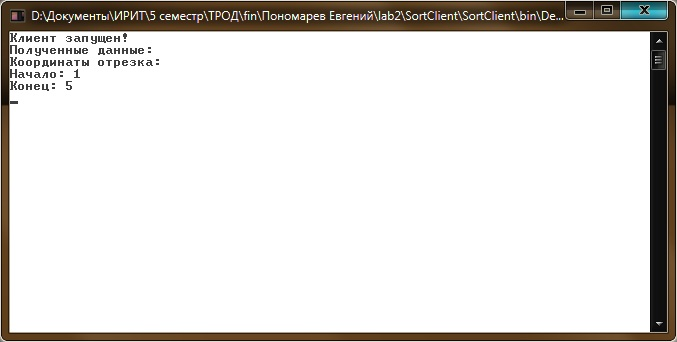
\includegraphics[scale = .5]{1-2}}
       		\caption{}
       		\label{ris:1-2}
       	\end{figure}
       	
       	Скриншот работы второго клиента представлен на Рис.\ref{ris:1-3}.
       	\begin{figure}[!h]
       		\centering{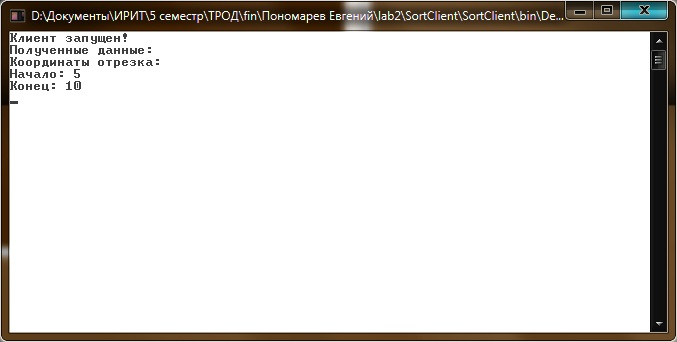
\includegraphics[scale = .5]{1-3}}
       		\caption{}
       		\label{ris:1-3}
       	\end{figure}
       	\newpage
       	Скриншот работы сервера представлен на Рис.\ref{ris:1-4}.
       	\begin{figure}[!h]
       		\centering{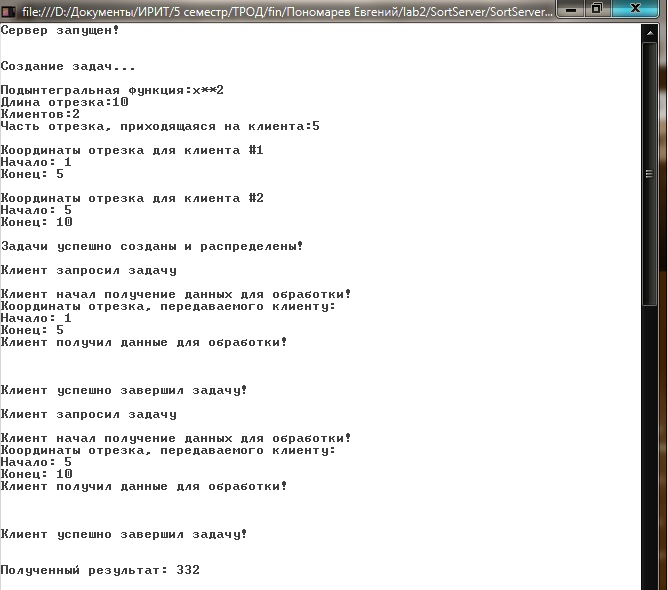
\includegraphics[scale = .6]{1-4}}
       		\caption{}
       		\label{ris:1-4}
       	\end{figure}
       	       	
	\section{Вывод}
	В результате выполнения лабораторной работы был получен программный комплекс, состоящий из сервера и клиента и реализующий алгоритм интегрирования методом Монте-Карло с использованием скрипта Python.
		
\end{document}